\documentclass{beamer}
\usepackage[latin1]{inputenc}
\usetheme{Warsaw}
\title[Volunteer Cloud Computing]{Volunteer Cloud Computing}
\author{Dany Wilson -- Stephane Some}
\institute{University of Ottawa}
\date{January 24, 2014}
\begin{document}

\begin{frame}
\titlepage
\end{frame}

\begin{frame}
  \frametitle{Agenda}
  \tableofcontents
\end{frame}

\section{Introduction}
\subsection{Volunteer Computing}
\begin{frame}
  \frametitle{Volunteer Computing}
  \begin{figure}[GIMPS]
    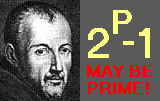
\includegraphics{GIMPS_logo.png}
  \end{figure}

  \begin{itemize}
  % Mersenne Prime numbers are prime numbers that are one less than a
  % power of 2  (3, 7, 31, 127)
  \item Great Internet Mersenne Prime Search [1996]
  \item Distributed Computing based on Collaboration
  \item ... throughput of 137.023 TeraFLOP/s
  \end{itemize}
\end{frame}

\subsection{Cloud Computing}

\begin{frame}
  \frametitle{Cloud Computing}
  \begin{itemize}
  \item Natural evolution of Web 2.0, SoA and Virtualization
    technologies. 
  \end{itemize}

  \begin{figure}[Cloud]
    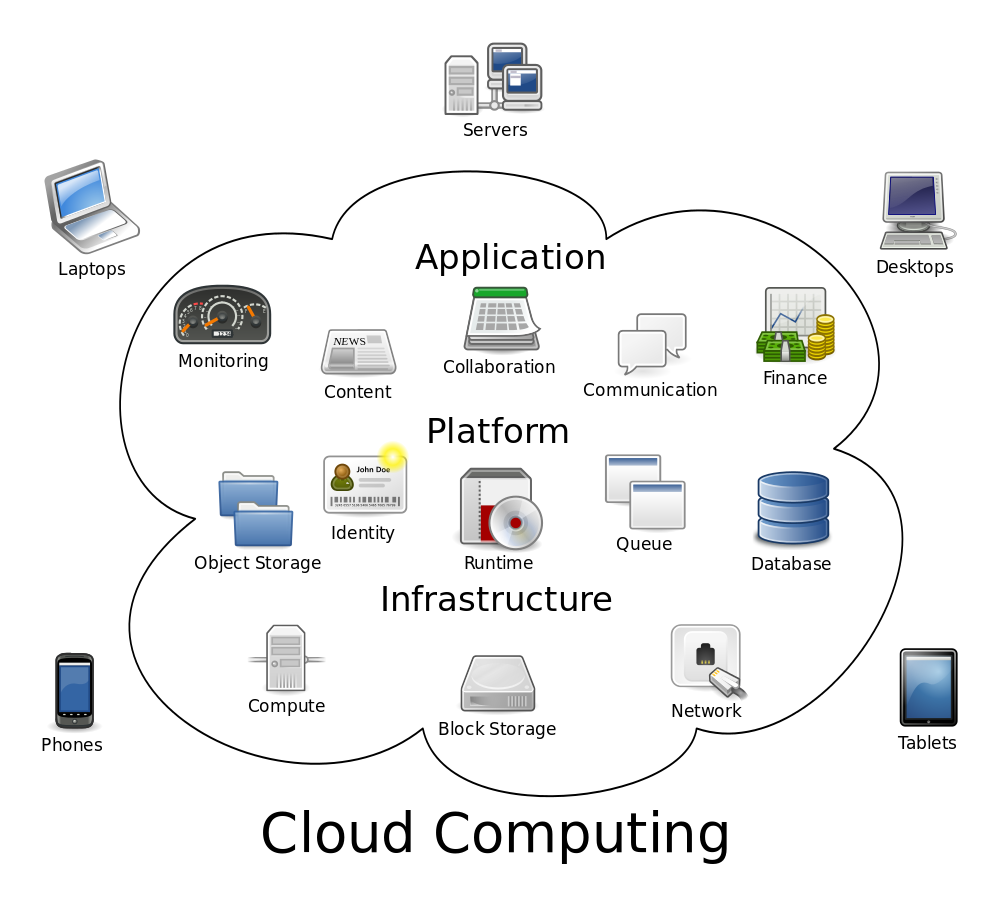
\includegraphics[width=\textwidth,height=0.8\textheight,keepaspectratio]{Cloud_computing.png}
  \end{figure}
\end{frame}

\begin{frame}
  \begin{figure}
    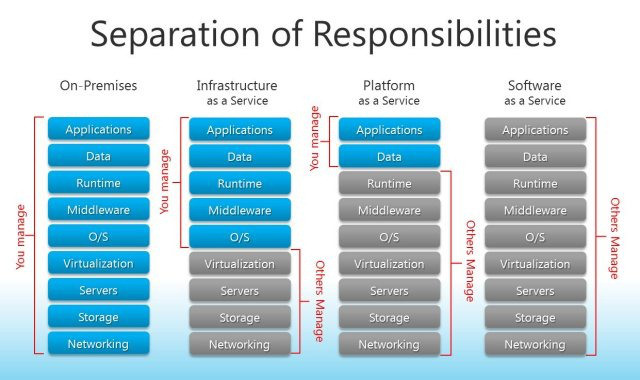
\includegraphics[width=\textwidth,height=0.8\textheight,keepaspectratio]{cloud_sep_of_resp.jpg}
  \end{figure}
\end{frame}

\subsection{Volunteer Cloud Computing}

\begin{frame}
  \frametitle{Volunteer Cloud Computing}
  \begin{itemize}
  \item Volunteer + Cloud = Volunteer Cloud Computing
  \end{itemize}
\end{frame}

\section{Related Work}
\begin{frame}
  \frametitle{Related Work}
  \begin{itemize}
  \item \textbf{Cloud@Home}[2009] and \textbf{Peer-2-Peer Cloud System}[2011]
  \item ... and a handful of conceptual reflections
  \end{itemize}
\end{frame}

\subsection{Cloud@Home}

\begin{frame}
 \frametitle{Cloud@Home}
     \begin{figure}[cathome]
      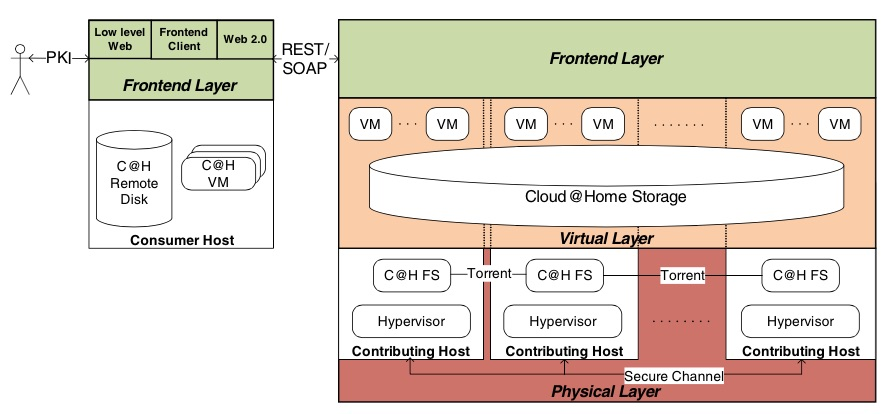
\includegraphics[width=\textwidth,height=0.8\textheight,keepaspectratio]{cathome_arch.jpg}
    \end{figure}
\end{frame}

\subsection{P2PCS}

\begin{frame}
  \frametitle{P2PCS}
  \begin{figure}
      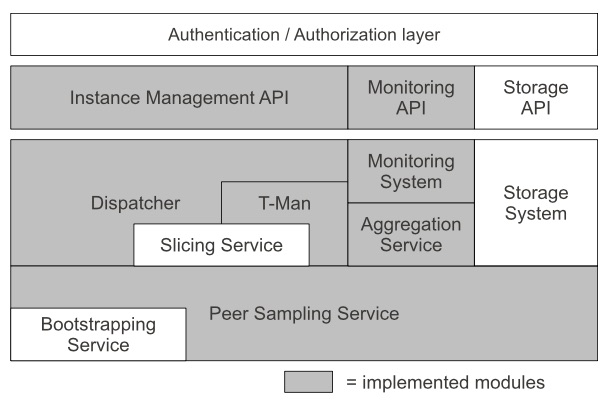
\includegraphics[width=\textwidth,height=0.8\textheight,keepaspectratio]{p2pcs_arch.jpg}
    \end{figure}
\end{frame}

\subsection{Analysis}

\begin{frame}
  \frametitle{Brief Analysis}
  \begin{itemize}
  \item \textbf{Scope}
  \item \textbf{Novelty} generally incurs under-specifications of the requirements!
  \end{itemize}
\end{frame}

\subsection{Requirements Definition}

\begin{frame}
  \frametitle{Requirements}
      \begin{figure}
      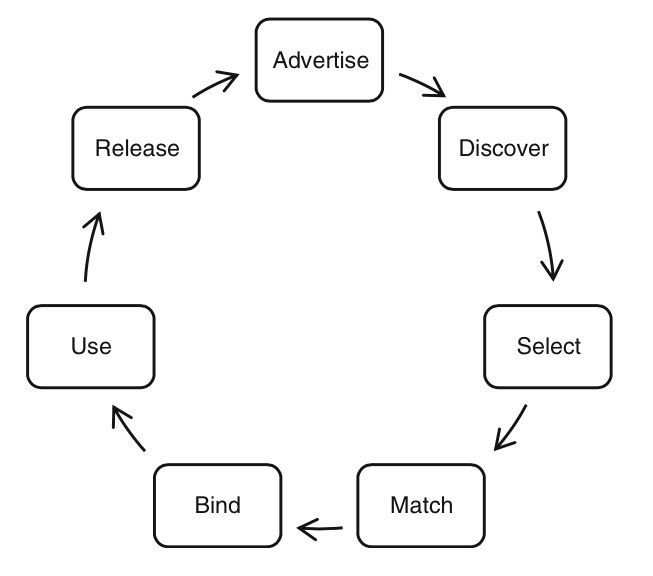
\includegraphics[width=\textwidth,height=0.8\textheight,keepaspectratio]{p2p-collab.jpg}
    \end{figure}
\end{frame}

\section{Infrastructure}
\begin{frame}
INFRASTRUCTURE 
\end{frame}  

\subsection{Overview}
\begin{frame}
  INFRASTRUCTURE
\end{frame}

\subsection{Physical Layer}
\begin{frame}
  INFRASTRUCTURE
\end{frame}

\subsection{Virtual Layer}
\begin{frame}
  INFRASTRUCTURE
\end{frame}

\subsection{API Layer}
\begin{frame}
  INFRASTRUCTURE
\end{frame}

\section{Open Problems}
\begin{frame}
  INFRASTRUCTURE
\end{frame}

\section{Future Work}
\begin{frame}
  INFRASTRUCTURE
\end{frame}

\section{Conclusion}
\begin{frame}
  INFRASTRUCTURE
\end{frame}

\section{References}
\begin{frame}
  INFRASTRUCTURE
\end{frame}

\end{document}
